\chapter{Looking into financial data}
%\addcontentsline{toc}{chapter}{Looking into real-world data}
\section{Five stocks and their evolution over 15 years}
We have chosen to study five stocks listed on the Paris Stock Exchange : BNP Paribas, Carrefour, LVMH, Sanofi and Total stocks.\footnote{We have chosen companies positioned on different domains, otherwise, information from different stock might more easily be redundant.} The evolution of the stock prices has been studied over the past 15 years, on a weekly basis. We first draw the data itself, then the net returns and the gross log returns on the stocks\footnote{Both quantities are widely used in Finance.}
\begin{figure}[h!]
	\centering
	\begin{minipage}[b]{0.4\textwidth}
 	\centering
 	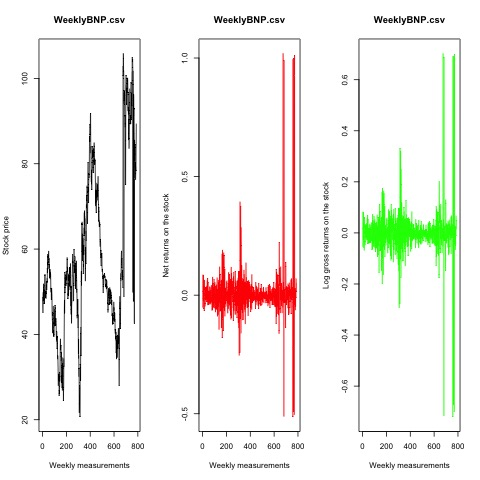
\includegraphics[scale = 0.4]{/Users/kimartin/Desktop/PDM_thesis_report/latex_template5_57/main/R_Files_3/WeeklyBNP.jpeg}
 	\caption{15 years of weekly BNP Stock Price Data}
 	\label{fig:BNPStock}
	\end{minipage}
	~
	\begin{minipage}[b]{0.4\textwidth}
  	\centering
  	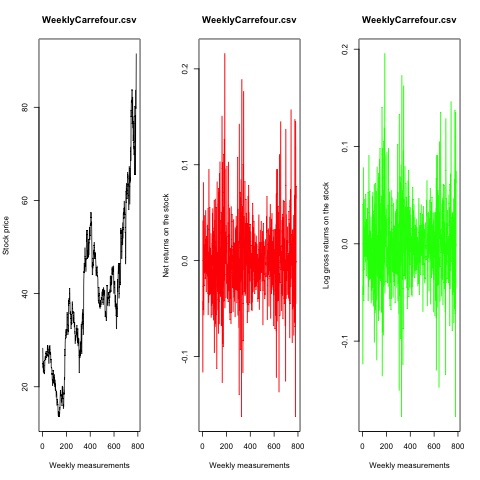
\includegraphics[scale = 0.4]{/Users/kimartin/Desktop/PDM_thesis_report/latex_template5_57/main/R_Files_3/WeeklyCarrefour.jpeg}
  	\caption{15 years of weekly Carrefour Stock Price Data}
  	\label{fig:CarrefourStock}
	\end{minipage}
\end{figure}
\begin{figure}[h!]
	\centering
	\begin{minipage}[b]{0.4\textwidth}
   	\centering
   	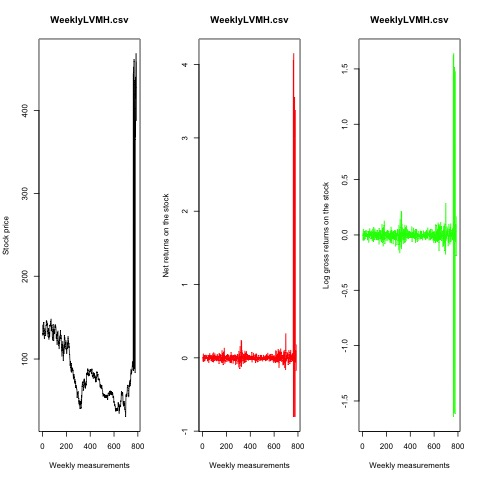
\includegraphics[scale = 0.4]{/Users/kimartin/Desktop/PDM_thesis_report/latex_template5_57/main/R_Files_3/WeeklyLVMH.jpeg}
   	\caption{15 years of weekly LVMH Stock Price Data}
   	\label{fig:LVMHStock}
	\end{minipage}
	~
	\begin{minipage}[b]{0.4\textwidth}
    	\centering
    	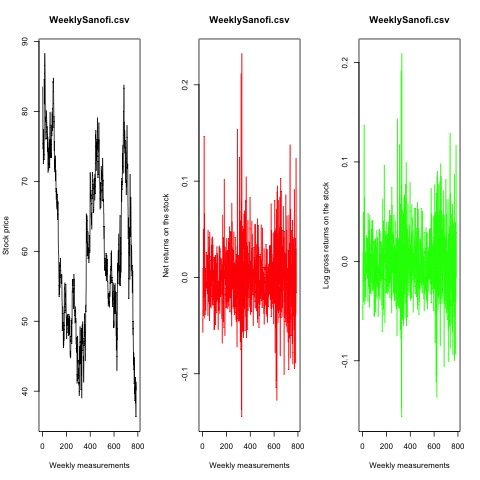
\includegraphics[scale = 0.4]{/Users/kimartin/Desktop/PDM_thesis_report/latex_template5_57/main/R_Files_3/WeeklySanofi.jpeg}
    	\caption{15 years of weekly Sanofi Stock Price Data}
    	\label{fig:SanofiStock}
	\end{minipage}
	~
	\begin{minipage}[b]{0.4\textwidth}
     	\centering
     	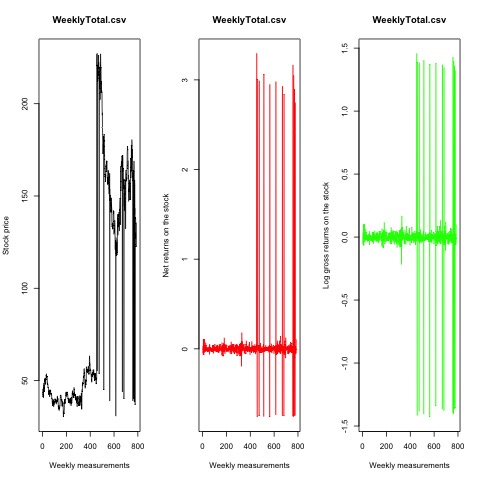
\includegraphics[scale = 0.4]{/Users/kimartin/Desktop/PDM_thesis_report/latex_template5_57/main/R_Files_3/WeeklyTotal.jpeg}
     	\caption{15 years of weekly Total Stock Price Data}
     	\label{fig:TotalStock}
	\end{minipage}
\end{figure}
\newpage
\paragraph{}
Let $X_t$ be the price of a stock at time $t$, the gross return at time $t + 1$ is defined as the ratio $\frac{X_{t+1}}{X_t}$, the net return at time $t + 1$ is defined as the ratio $r_t = \frac{X_{t+1}-X_t}{X_t}$ and the log gross return at time $t +1$ is defined as the log of the gross return at time $t + 1$ i.e. $R_t = \log(\frac{X_{t+1}}{X_t})$. The latter two quantities are of particular interest in Finance. 
\newline
Let us observe that the relationship between $R_t$, $X_t$ and $X_{t+1}$ can be rewritten as $X_{t+1} = \exp(R_{t+1}) X_t$. An approximation would be to take $X_{t+1} = (1 + R_{t+1}) X_t$ by taking the expansion of the exponential, cut at order 1. Below are the plots of the quantities $\exp(R_t)$ and $1 + R_t$ for the five stocks previously considered. As we can see from the value of the residuals (of order 1E-15\footnote{report to the appendix 'Additional figures' for the details.}), this is in practice a very good approximation !
\begin{figure}[h!]
	\centering
	\begin{minipage}[b]{0.4\textwidth}
		\centering
		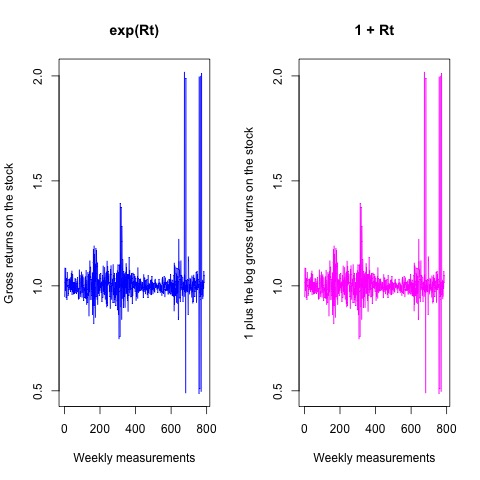
\includegraphics[scale = 0.425]{/Users/kimartin/Desktop/PDM_thesis_report/latex_template5_57/main/R_Files_3/WeeklyBNP_1+Rt_eRt.jpeg}
		\caption{$\exp(R_t)$ and $1 + R_t$ for BNP Stock Price Data}
		\label{fig:BNPCompApproxStock}
	\end{minipage}
	~
	\begin{minipage}[b]{0.4\textwidth}
		\centering
		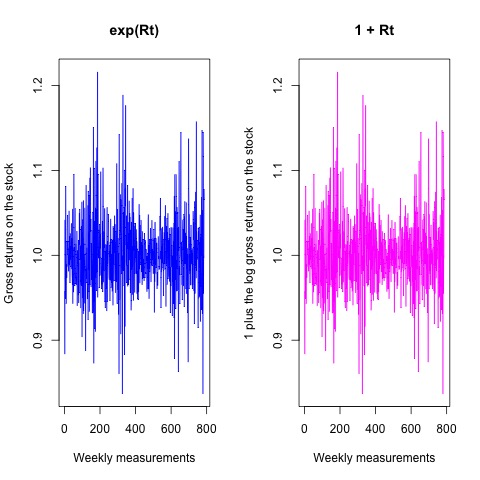
\includegraphics[scale = 0.425]{/Users/kimartin/Desktop/PDM_thesis_report/latex_template5_57/main/R_Files_3/WeeklyCarrefour_1+Rt_eRt.jpeg}
		\caption{$\exp(R_t)$ and $1 + R_t$ for Carrefour Stock Price Data}
		\label{fig:CarrefourCompApproxStock}
	\end{minipage}
\end{figure}
\\
\begin{figure}[h!]
	\centering
	\begin{minipage}[b]{0.4\textwidth}
		\centering
		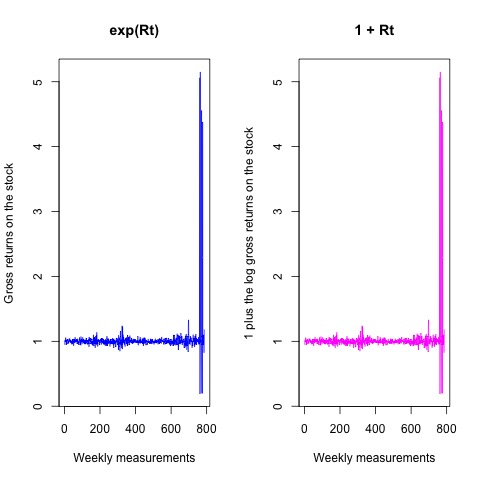
\includegraphics[scale = 0.425]{/Users/kimartin/Desktop/PDM_thesis_report/latex_template5_57/main/R_Files_3/WeeklyLVMH_1+Rt_eRt.jpeg}
		\caption{$\exp(R_t)$ and $1 + R_t$ for LVMH Stock Price Data}
		\label{fig:LVMHCompApproxStock}
	\end{minipage}
	~
	\begin{minipage}[b]{0.4\textwidth}
		\centering
		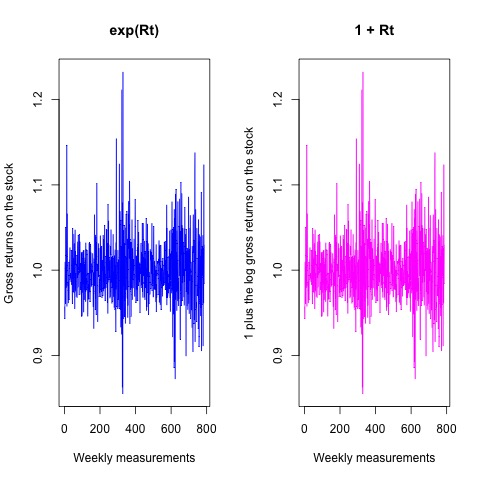
\includegraphics[scale = 0.425]{/Users/kimartin/Desktop/PDM_thesis_report/latex_template5_57/main/R_Files_3/WeeklySanofi_1+Rt_eRt.jpeg}
		\caption{$\exp(R_t)$ and $1 + R_t$ for Sanofi Stock Price Data}
		\label{fig:SanofiCompApproxStock}
	\end{minipage}
\end{figure}
\\
\begin{figure}[h!]
	\centering
	\begin{minipage}[b]{0.4\textwidth}
		\centering
		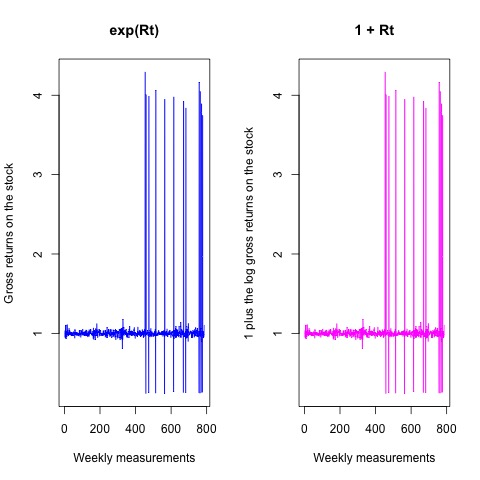
\includegraphics[scale = 0.425]{/Users/kimartin/Desktop/PDM_thesis_report/latex_template5_57/main/R_Files_3/WeeklyTotal_1+Rt_eRt.jpeg}
		\caption{$\exp(R_t)$ and $1 + R_t$ for Total Stock Price Data}
		\label{fig:TotalCompApproxStock}
	\end{minipage}
\end{figure}
\\


\section{A détour around Stochastic Calculus}
\subsection{The Black-Scholes Stochastic Differential Equation}
\paragraph{Presentation}
It is customary to model the evolution of stock prices by a stochastic process $(S_t)_{t \ge 0}$ satisfying the Black-Scholes stochastic differential equation\footnote{Actually, a first model could be as simple as using arithmetical random walks. Two problems would however arise. The first is that if we used an ARW we could get negative stock prices, the second problem is that stocks selling at low prices usually have low price increments while stocks selling at high prices usually have larger price increments. In the Black-Scholes model, the price increment at time $t+1$ is made up of a component proportional to the price at time $t$ and a stochastic component. The stochastic component is also proportional to the price at time $t$. Both problems are thus solved. The process $(S_t)_{t \ge 0}$ is continuous and when $S_t$ reaches $0$, the infinitesimal increment which is $S_t (\mu \mathrm{d}t + \sigma \mathrm{d}B_t )$ is also $0$. Therefore, $S_t$ cannot go below $0$.}, which rea\mathrm{d}s as follows : 
\begin{equation}
\mathrm{d}S_t = \mu S_t \mathrm{d}t + \sigma S_t \mathrm{d}B_t
\end{equation}
where $(B_t)_{t \ge 0}$ is a standard Brownian Motion with respect to a filtration $({\cal{F}}_t)_{t \ge 0}$. Let us observe that the stochastic differential equation above is the Black-Scholes SDE with time independent coefficients : both the drift $\mu \in \mathbb{R}$ and the volatility $\sigma > 0$ are constant.\footnote{In the next subsection, we will deal with the Black-Scholes SDE with time dependent coefficients.} An initial condition must be specified : $S_0 = s_0 > 0$.
\paragraph{Resolution - existence of a solution to the Black-Scholes SDE}
Let us consider the following generic stochastic differential equation : \\
$\left\{
\begin{array}{l}
\mathrm{d}X_t = f(X_t) \mathrm{d}t + g(X_t) \mathrm{d}B_t\\
X_0 = x_0
\end{array}
\right.$ \\ where $(B_t)_{t \ge 0}$ is a standard Brownian Motion with respect to a filtration $({\cal{F}}_t)_{t \ge 0}$, $x_0 \in \mathbb{R}$, $f,g : \mathbb{R} \longrightarrow \mathbb{R}$ are Lipschitz functions. Then, by a theorem from Stochastic Calculus\footnote{readers wanting to get ahold of an excellent course on Stochastic Calculus are advised to refer to Dr. Lév\^{e}que's course. It can be found at \url{http://ipg.epfl.ch/~leveque/}}, we know that there exists a unique process that is continuous and adapted to the filtration $({\cal{F}}_t)_{t \ge 0}$. \\
Here, f and g are respectively the functions $x \longrightarrow \mu x$ and $x \longrightarrow \sigma t$. These functions are Lipschitz functions, therefore we know the SDE admits a solution. And fortunately, in the case of the Black-Scholes equation, the solution can be made explicit\footnote{This is not always the case : solving SDEs in general is not that simple, and finding an explicit solution is not guaranteed in the general case, even though we know one exists.}).
\paragraph{Resolution - step 1}
Let us set $S_t = \phi_t Z_t$ where $\phi_t$ is the (deterministic) solution to the ordinary differential equation :
\\
$\left\{
\begin{array}{l}
\mathrm{d}\phi_t = \mu \phi_t \mathrm{d}t\\
\phi_0 = 1
\end{array}
\right.$ \\ Solving this ODE is elementary and yiel\mathrm{d}s the solution $\phi_t = \exp(\mu t)$. Now, let us differentiate $X_t$ under its form as a product  $S_t = \phi_t Z_t$. \\
\begin{equation}
\begin{alignat*}{2}
\mathrm{d}(S_t) &= \mathrm{d}(\phi_t Z_t)\\ 
&= \phi_t \mathrm{d}Z_t + Z_t \mathrm{d}\phi_t + \mathrm{d}<\phi,Z>_t\\ 
&= \phi_t \mathrm{d}Z_t + \mu \phi_t Z_t \mathrm{d}t\\
&= \phi_t \mathrm{d}Z_t + \mu S_t \mathrm{d}t\\
\end{alignat*}
\end{equation} where the infinitesimal quadratic covariation between $\phi$ and $Z$ is zero as $\phi$ has bounded variations. If we compare the last right-hand term of the series of equations just above to the original Black-Scholes SDE, we see that $\sigma S_t \mathrm{d}B_t = \phi_t \mathrm{d}Z_t$. Hence, $\mathrm{d}Z_t = \sigma Z_t \mathrm{d}B_t$. Here, we must be very careful as this differential equation does not integrate as it would in the settings of 'usual' calculus, in particular, integrating it to $\log(Z_t) - \log(Z_0) = \sigma (B_t - B_0)$ is \underline{totally wrong !}
\paragraph{Resolution - step 2}
Now, let us set $Y_t = \log(Z_t)$. Using Ito-Doeblin's formula, we get : \\
$d(\log(Z_t)) = \frac{1}{Z_t} \mathrm{d}Z_t + \frac{1}{2} (\frac{-1}{Z^2_{t}})\mathrm{d}<Z>_t$ ($\star$)\\
\underline{$\rightarrow$ How to compute $\mathrm{d}<Z>_t$ ?}
\begin{equation}
\begin{alignat*}{2}
S_t &= \phi_t Z_t\\ 
\implies Z_t &= \frac{S_t}{\phi_t}\\ 
\implies \mathrm{d}Z_t &= \frac{1}{\phi_t} \mathrm{d}S_t + S_t d(\frac{1}{\phi_t}) + \mathrm{d}<\frac{1}{\phi},S>_t\\
&= \frac{1}{\phi_t} \mathrm{d}S_t - \frac{S_t}{\phi_t^2} d(\phi_t) \\
&= \frac{1}{\phi_t} \mathrm{d}S_t - \frac{\mu S_t}{\phi_t} \mathrm{d}t \\
&= \frac{1}{\phi_t} (\mu S_t \mathrm{d}t + \sigma S_t \mathrm{d}B_t) - \frac{\mu S_t}{\phi_t} \mathrm{d}t \\
&= \frac{\sigma S_t}{\phi_t} \mathrm{d}B_t 
\end{alignat*}
\end{equation} where the infinitesimal quadratic covariation between $\frac{1}{\phi}$ and $Z$ is zero as $\frac{1}{\phi}$ has bounded variations, in the third equality from the top.\newline
Hence, using the Isometry formula, we have that :
\begin{alignat*}{2}
<Z>_t &= \int_0^t \! \frac{\sigma^2 S_s^2}{\phi_s^2} \, \mathrm{d}s \\ 
 &= \int_0^t \! \sigma^2 Z_s^2 \, \mathrm{d}s \\ 
\implies \mathrm{d}<Z>_t &= \sigma^2 Z_t^2 \mathrm{d}t
\end{alignat*}
\end{equation} \newline
Back to ($\star$), we now have :
\begin{equation}
\begin{alignat*}{2}
\mathrm{d}(\log(Z_t)) &= \frac{1}{Z_t} \mathrm{d}Z_t + \frac{1}{2} (\frac{-1}{Z^2_{t}}) \sigma^2 Z^2_{t} \mathrm{d}t \\
\iff \frac{1}{Z_t} \mathrm{d}Z_t &= d(\log(Z_t)) + \frac{\sigma^2}{2} \mathrm{d}t 
\end{alignat*}
\end{equation} 
\paragraph{Resolution - step 3}
Combining the previous equation with $\mathrm{d}Z_t = \sigma Z_t \mathrm{d}B_t$, we get : \newline
\begin{equation}
\begin{alignat*}{2}
\sigma \mathrm{d}B_t &= \mathrm{d}(log(Z_t)) + \frac{\sigma^2}{2} \mathrm{d}t \\
\implies \log(Z_t) -\log(Z_0) &= -\frac{\sigma^2}{2} (t - 0) + \sigma (B_t - B_0) \\
\implies \log(Z_t) -\log(\frac{S_0}{\phi_0}) &= -\frac{\sigma^2}{2} t + \sigma B_t \\
\implies \log(Z_t) &= \log(s_0) -\frac{\sigma^2}{2} t + \sigma B_t \\
\implies Z_t &= s_0 \exp(-\frac{\sigma^2}{2} t + \sigma B_t )
\end{alignat*}
\end{equation} \newline Finally, by remembering that $S_t = \phi_t Z_t = \exp(\mu t) Z_t$, we get :\newline
$\forall t \ge 0, S_t = s_0 \exp((\mu -\frac{\sigma^2}{2}) t + \sigma B_t)$
\newline The stochastic process $(S_t)_{t \ge 0}$, made explicit above, that is solution to the Black-Scholes equation is generally called Geometric Brownian Motion in the literature.
\subsection{Black-Scholes SDE with time-dependent coefficients }
\paragraph{Presentation} In the simple Black-Scholes SDE, the drift $\mu$ and the volatility $\sigma$ were time-independent constants. Let us now consider a more general version of the Black-Scholes SDE : \newline
$\left\{
\begin{array}{l}
\mathrm{d}S_t = \mu(t) S_t \mathrm{d}t + \sigma(t) S_t \mathrm{d}B_t\\
S_0 = s_0 > 0
\end{array}
\right.$ \newline where $(B_t)_{t \ge 0}$ is a standard Brownian Motion with respect to a filtration $({\cal{F}}_t)_{t \ge 0}$, $\mu, \sigma$ two continuous functions such that there exists $K_1 > 0$, $K_2 > 0$, such that $\forall t \ge 0$, $\lvert \mu(t) \rvert \le K_1$, $K_2 \le \lvert \sigma(t) \rvert \le K_1$.
\paragraph{Resolution - existence of a solution to the generalized Black-Scholes SDE}
Let us consider the following generic stochastic differential equation : \\
$\left\{
\begin{array}{l}
\mathrm{d}X_t = f(t,X_t) \mathrm{d}t + g(t,X_t) \mathrm{d}B_t\\
X_0 = x_0
\end{array}
\right.$ \\ where $(B_t)_{t \ge 0}$ is a standard Brownian Motion with respect to a filtration $({\cal{F}}_t)_{t \ge 0}$, $x_0 \in \mathbb{R}$, $f,g : \mathbb{R}_{+} \times \mathbb{R} \longrightarrow \mathbb{R}$ are jointly continuous in $(t,x)$ and Lipschitz in x. Then, by a theorem from Stochastic Calculus, we know that there exists a unique solution $(X_t)_{t \ge 0}$ to the SDE. in the case of the generalized Black-Scholes SDE, the conditions are met and we can thus conclude that it admits a unique solution. The solution can be made explicit here too, fortunately !
\paragraph{Resolution}
Let us set $Y_t = \log(S_t)$, we then have $\mathrm{d}Y_t = \frac{1}{S_t}\mathrm{d}S_t -\frac{1}{2} \frac{1}{S_t^2} \mathrm{d}<S>_t$. If we remember that $\mathrm{d}S_t = \mu(t) S_t \mathrm{d}t + \sigma(t) S_t \mathrm{d}B_t$ and apply the Isometry formula, we get that $\mathrm{d}<S>_t = \sigma(t)^2 X_t^2 \mathrm{d}t$. We thus get : \newline
\begin{equation}
\begin{alignat*}{2}
\sigma \mathrm{d}Y_t &= \frac{1}{S_t} \mathrm{d}S_t - \frac{1}{2} \frac{1}{S_t^2} \mathrm{d}<S>_t \\
&=  \frac{1}{S_t} \mathrm{d}S_t - \frac{1}{2} \sigma(t)^2 \mathrm{d}t \\
&=  \frac{1}{S_t} (\mu(t) S_t \mathrm{d}t + \sigma(t) S_t \mathrm{d}B_t)- \frac{1}{2} \sigma(t)^2 \mathrm{d}t \\
 &= (\mu(t) - \frac{1}{2} \sigma(t)^2) \mathrm{d}t + \sigma(t) dBt \\
\implies Y_t &= y_0 + \int_0^t \! (\mu(s) - \frac{1}{2} \sigma(s)^2) \, \mathrm{d}s + \int_0^t \! \sigma(s) \, \mathrm{d}B_s \\
\implies Y_t &= \log(s_0) + \int_0^t \! (\mu(s) - \frac{1}{2} \sigma(s)^2) \, \mathrm{d}s + \int_0^t \! \sigma(s) \, \mathrm{d}B_s \\
\implies S_t &= s_0 \exp(\int_0^t \! (\mu(s) - \frac{1}{2} \sigma(s)^2) \, \mathrm{d}s + \int_0^t \! \sigma(s) \, \mathrm{d}B_s)  \\
\end{alignat*}
\end{equation}\newline
Let us observe that the solution found in the case of the generalized Black-Scholes SDE is coherent with the solution found for the simple Black-Scholes SDE\footnote{Just set functions $\mu$ and $\sigma$ equal to constants $\mu$ and $\sigma$ and we are back with the Geometric Brownian Motion previously found. }.

\section{Back to the data}
\paragraph{Fitting the data to the model} We are now going to assume the stock prices $S_t^{(i)}$\footnote{The notations are the following :\newline \begin{itemize}
		\item $S_t^{(1)}$ for the BNP stock.
		\item $S_t^{(2)}$ for the Carrefour stock.
		\item $S_t^{(3)}$ for the LVMH stock.
		\item $S_t^{(4)}$ for the Sanofi stock.
		\item $S_t^{(5)}$ for the Total stock.
	\end{itemize}} we have been studying follow the (simple) Black-Scholes model that is that their prices can be modeled by a geometric brownian motion. We will determine the corresponding $\mu_i$'s and $\sigma_i$'s. To do that, we will make explicit the gross return at time $t + 1$ : \newline
\begin{equation}
\begin{alignat*}{2}
\frac{S_{t + 1}}{S_t} &= \frac{s_0 \exp((\mu -\frac{\sigma^2}{2}) (t + 1) + \sigma B_{t + 1}}{s_0 \exp((\mu -\frac{\sigma^2}{2}) t + \sigma B_t)} \\
\implies \frac{S_{t + 1}}{S_t} &= \exp(\mu -\frac{\sigma^2}{2}) \exp(\sigma (B_{t + 1} - B_t))
\end{alignat*}
\end{equation}\newline	
A first observation that we could make is that as $x \longrightarrow \exp(\sigma x)$ is a Borel-measurable function (because it is continuous) and the increments of the brownian motion are independent, $\frac{S_{t}}{S_{t - 1}} &= \exp(\mu -\frac{\sigma^2}{2}) \exp(\sigma (B_{t} - B_{t - 1}))$ and $S_t = s_0 \exp((\mu -\frac{\sigma^2}{2}) t + \sigma B_t) = s_0 \exp((\mu -\frac{\sigma^2}{2}) t + \sigma (B_t - B_0))$ are independent $\forall t \ge 0 $.\footnote{This is the formal justification behind the well-known fact that under the Black-Scholes model, the gross return at a time step is independent of the price of the stock at that date.} Let us now consider the log-gross returns $R_t = (\mu -\frac{\sigma^2}{2}) + (\sigma (B_{t} - B_{t - 1}))$. It is thus easy to see that $R_t$ has a gaussian distribution $\mathcal{N}((\mu -\frac{\sigma^2}{2}), \sigma^2)$. Therefore, to find the $\mu_i$'s and $\sigma_i$'s, we just have to compute the mean and the variance of the empirical log-gross returns which we respectively denote by $\mu_{EMP}$ and $\sigma_{EMP}^2$.
\begin{equation}
\begin{alignat*}{2}
\begin{cases} \sigma^2 &= \sigma_{EMP}^2\\
\mu &= \mu_{EMP} + \frac{\sigma_{EMP}^2}{2} \end{cases}
\end{alignat*}
\end{equation}\newline	
\newpage
\begin{figure}[h!]
	\centering
		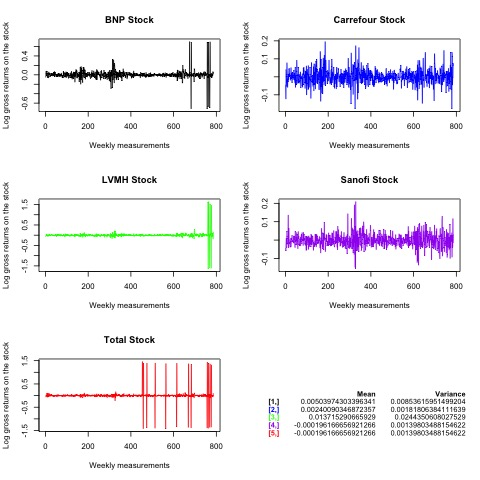
\includegraphics[scale = 1]{/Users/kimartin/Desktop/PDM_github_repo/pdmExtremeValueTheory/r_files_logGrossReturns/logGrossReturns.jpeg}
		\caption{Log-gross returns on the stock, the $\mu$'s and the $\sigma^2$'s.}
		\label{fig:LogGrossReturns}
\end{figure}
Now that we have the $\mu$'s and the $\sigma^2$'s for the stocks, we will simulate geometric Brownian motions with these parameters, and compare the results to the original data. We will run several, say 5, simulations and make a few observations. Below the corresponding plots can be found with the \textbf{yellow line representing each time the simulated geometric Brownian motion} :
%\begin{itemize}
	%\item \textbf{First} plotted the actual stock prices, each paired with the corresponding simulated geometric Brownian motion.
	%\item \textbf{Second} plotted the actual stock prices, each paired with an average of 100 corresponding simulated geometric Brownian motions.
%\end{itemize}
\begin{figure}[h!]
	\centering
	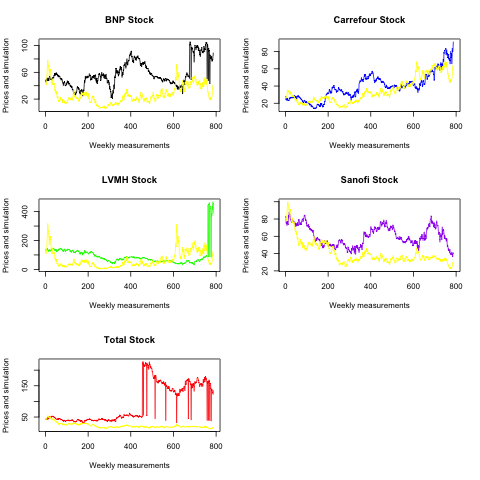
\includegraphics[scale = 1]{/Users/kimartin/Desktop/PDM_github_repo/pdmExtremeValueTheory/r_files_logGrossReturns/actualAndSimulatedRescaledA.png}
	\caption{The actual stock prices and a 1$^{st}$ simulation of the corresponding geometric Brownian motions.}
	\label{fig:ActualAndSimulatedGeomBMs1}
\end{figure}
\newpage
\begin{figure}[h!]
	\centering
	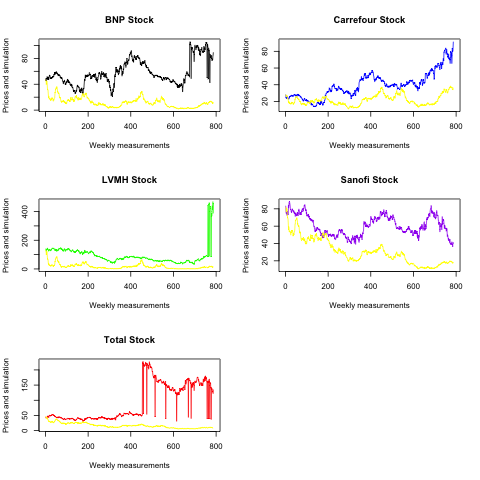
\includegraphics[scale = 1]{/Users/kimartin/Desktop/PDM_github_repo/pdmExtremeValueTheory/r_files_logGrossReturns/actualAndSimulatedRescaledB.png}
	\caption{The actual stock prices and a 2$^{nd}$ simulation of the corresponding geometric Brownian motions.}
	\label{fig:ActualAndManySimulatedGeomBMs2}
\end{figure}
\newpage
\begin{figure}[h!]
	\centering
	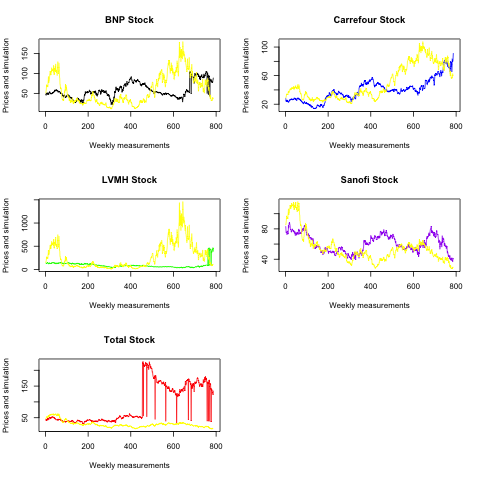
\includegraphics[scale = 1]{/Users/kimartin/Desktop/PDM_github_repo/pdmExtremeValueTheory/r_files_logGrossReturns/actualAndSimulatedRescaledC.png}
	\caption{The actual stock prices and a 3$^{rd}$ simulation of the corresponding geometric Brownian motions.}
	\label{fig:ActualAndManySimulatedGeomBMs3}
\end{figure}
\newpage
\begin{figure}[h!]
	\centering
	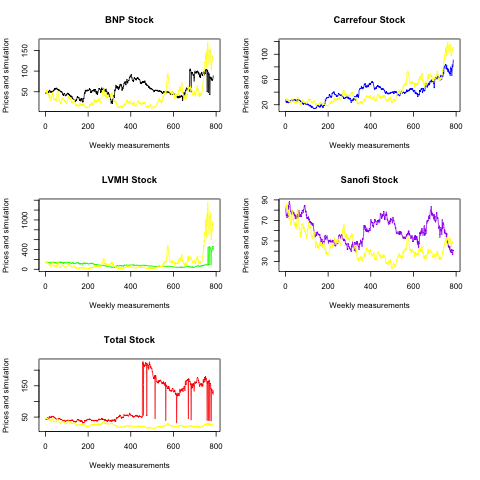
\includegraphics[scale = 1]{/Users/kimartin/Desktop/PDM_github_repo/pdmExtremeValueTheory/r_files_logGrossReturns/actualAndSimulatedRescaledD.png}
	\caption{The actual stock prices and a 4$^{th}$ simulation of the corresponding geometric Brownian motions.}
	\label{fig:ActualAndManySimulatedGeomBMs4}
\end{figure}
\newpage
\begin{figure}[h!]
	\centering
	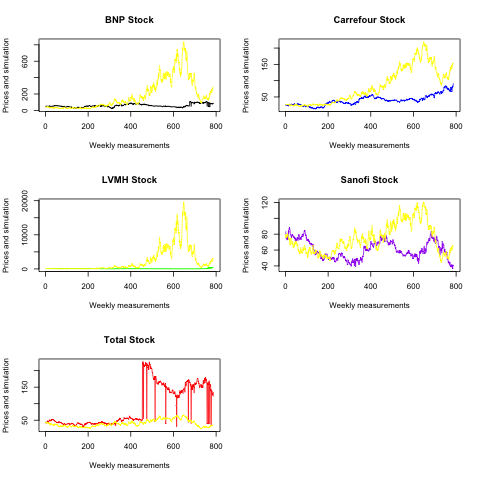
\includegraphics[scale = 1]{/Users/kimartin/Desktop/PDM_github_repo/pdmExtremeValueTheory/r_files_logGrossReturns/actualAndSimulatedRescaledE.png}
	\caption{The actual stock prices and a 5$^{th}$ simulation of the corresponding geometric Brownian motions.}
	\label{fig:ActualAndManySimulatedGeomBMs5}
\end{figure}
\clearpage
\subsection{Observations}
As we can see, using a geometric Brownian motion to model stock prices yields rather good results though the last simulation displays a case of (gross) overestimation of the prices. However, let us note that this true for the BNP, Carrefour and Sanofi stocks. If we have a look at the Total stock, we see that from week 500 or so the stock price varies quickly widely. The geometric Brownian motion is unable to cope with this behaviour, all five simulations are outright failures. There is a similar issue with the LVMH stock at the end of the series after a rather flat behaviour for most of the duration of the observations, which may explain why the simulations are poor in the case of that stock too. \newline
As a consequence, we have decided to cut the LVMH and Total data so as to keep only the part of the time series where the stock prices are not too volatile, and then apply our simulation to the cut time series. As we can see below, the result is better\footnote{The LVMH stock, though, is still more volatile than the Total stock. That explains why the simulation is poorer for the former than for the latter.}
\begin{figure}[h!]
	\centering
	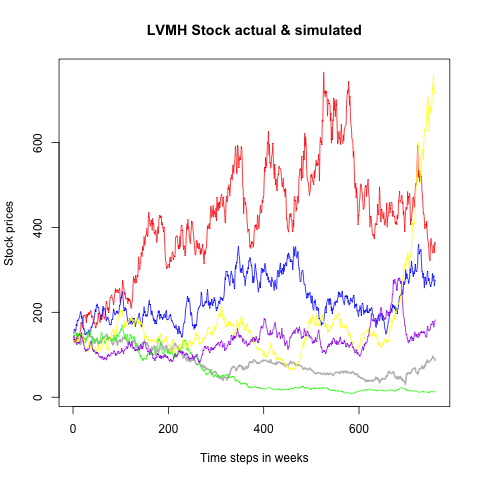
\includegraphics[scale = 1]{/Users/kimartin/Desktop/R_files_pdm/Tache7/cleanedLVMH.png}
	\caption{Cut LVMH stock price time series. In \textbf{grey} the actual prices, in colour five different runs of the simulation}
	\label{fig:cutLVMH}
\end{figure}
\begin{figure}[h!]
	\centering
	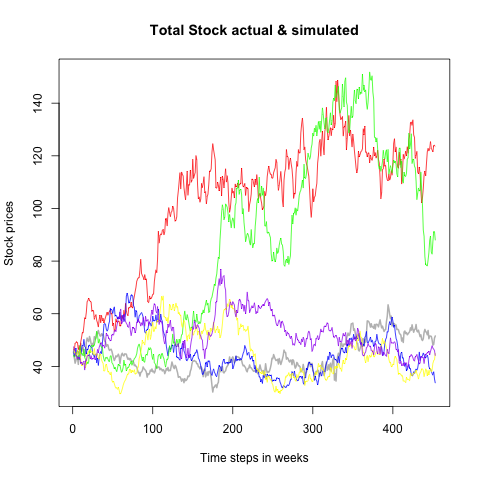
\includegraphics[scale = 1]{/Users/kimartin/Desktop/R_files_pdm/Tache7/cleanedTotal.png}
	\caption{Cut Total stock price time series. In \textbf{grey} the actual prices, in colour five different runs of the simulation}
	\label{fig:cutTotal}
\end{figure}
\clearpage
We can even get a better simulation if we choose a smaller time increment for it : the actual data is weekly, but in our simulation we can choose to take a daily time increment if we so desire. As shown below, it improves a bit the quality of the simulation.
\begin{figure}[h!]
	\centering
	\includegraphics[scale = 0.85]{/Users/kimartin/Desktop/R_files_pdm/Tache7/cleanedLVMH_better_simulation_copy.png}
	\caption{Cut LVMH stock price time series. In \textbf{grey} the actual weekly prices, in colour two runs of the daily simulation}
	\label{fig:cutLVMHbetter}
\end{figure}
\begin{figure}[h!]
	\centering
	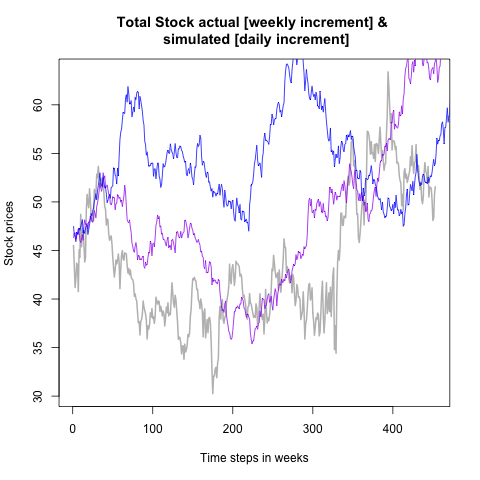
\includegraphics[scale = 0.85]{/Users/kimartin/Desktop/R_files_pdm/Tache7/cleanedTotal_better_simulation.png}
	\caption{Cut Total stock price time series. In \textbf{grey} the actual weekly prices, in colour two runs of the daily simulation}
	\label{fig:cutTotalbetter}
\end{figure}
\clearpage
\section{Fitting data above a threshold}
Finally, we are going to try and fit a generalised extreme value distribution to our data. For each stock, we keep only the data that is above the empirical $95$ \%-quantile. We then call the function \textit{gev.fit} and \textit{gev.diag} from the R package \textit{ismev}. We are particularly interested in the density plot thus obtained, as they will allow to conclude as to the distribution fitting the data.
\begin{figure}[h!]
	\centering
	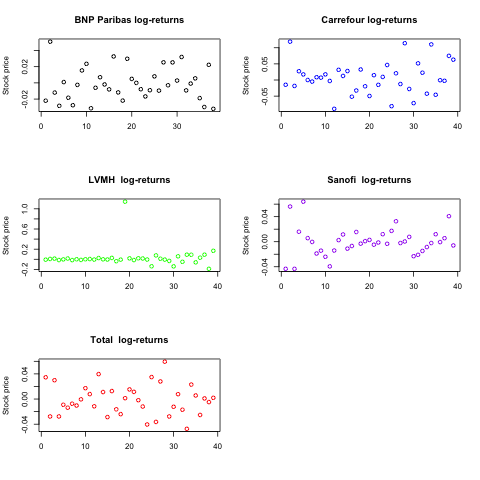
\includegraphics[scale = 1]{/Users/kimartin/Desktop/PDM_github_repo/pdmExtremeValueTheory/r_files_tache8/aboveThresholdData.png}
	\caption{Data above the  $95$ \%-quantile for the BNP Paribas, Carrefour, LVMH, Sanofi and Total stocks.}
	\label{fig:dataAboveThreshold}
\end{figure}
\clearpage
The pattern followed by the LVMH data is most dissimilar to that followed by the other stocks. It suggests that the fitting may yield poor results. 
\paragraph{BNP Paribas stock }
\begin{figure}[h!]
	\centering
	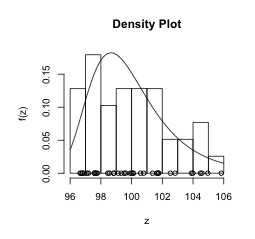
\includegraphics[scale = 1]{/Users/kimartin/Desktop/PDM_github_repo/pdmExtremeValueTheory/r_files_tache8/BNP_Paribas_fitted}
	\caption{Density fitting for the BNP Paribas data \\}
	\label{fig:dataAboveThresholdBNPFitted}
\end{figure}
\paragraph{Carrefour stock }
\begin{figure}[h!]
	\centering
	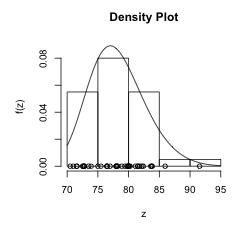
\includegraphics[scale = 1]{/Users/kimartin/Desktop/PDM_github_repo/pdmExtremeValueTheory/r_files_tache8/Carrefour_fitted}
	\caption{Density fitting for the Carrefour data \\}
	\label{fig:dataAboveThresholdBNPFitted}
\end{figure}
\paragraph{Sanofi stock}
\begin{figure}[h!]
	\centering
	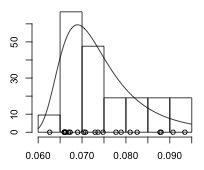
\includegraphics[scale = 1]{/Users/kimartin/Desktop/PDM_github_repo/pdmExtremeValueTheory/r_files_tache8/Sanofi_fitted}
	\caption{Density fitting for the Sanofi data \\}
	\label{fig:dataAboveThresholdSanofiFitted}
\end{figure}
\paragraph{Total stock}
\begin{figure}[h!]
	\centering
	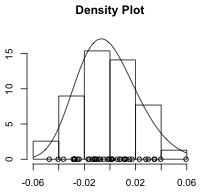
\includegraphics[scale = 1]{/Users/kimartin/Desktop/PDM_github_repo/pdmExtremeValueTheory/r_files_tache8/Total_fitted}
	\caption{Density fitting for the Total data \\}
	\label{fig:dataAboveThresholdtotalFitted}
\end{figure}
\paragraph{LVMH stock}
\begin{figure}[h!]
	\centering
	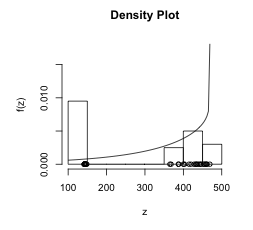
\includegraphics[scale = 1]{/Users/kimartin/Desktop/PDM_github_repo/pdmExtremeValueTheory/r_files_tache8/LVMH_fitted}
	\caption{Density fitting for the LVMH data \\}
	\label{fig:dataAboveThresholdLVMHFitted}
\end{figure}